% !TeX root = ../report.tex

% Key information to be included:
% - Few lines about the general method and the steps followed
% - Heuristics (report the definitions in the previous slides)
% - Metrics agreed among all evaluators
% - Final scores agreed among all evaluators (include the main comments
% for your scores and examples of commentedscreenshots to support
% your scores)
% - Annex: Report the scores and main comments of EACH evaluator
% - PROVIDE AGGREGATED DATA, e.g., MEAN VALUES FOR ALL EURISTICS,
% (MEAN) SCORE BY DIMENSIONS (e.g., for CONTENT HEURISTICS,
% NAVIGATION HEURISTICS, ect.)
% - PROVIDE VISUAL REPRESENTATIONS OF RESULTS (diagrams, summary
% tables...)
% - Include a short conclusion section where you breifly discuss inspection
% results

\section{Inspection}

\subsection{Method}
% what is inspection based usability evaluation
% specific heuristics and metrics used
Inspection-based usability evaluation allows teams of evaluators to perform
a systemic analisys of UI/UX aspects of an application (a website, in our case).
We adopted the widely used \emph{heuristic evaluation}, as the main usability inspection method, in which the evaluators concentrate on a set of principles (``heuristics'') to test the usability of the application.

\subsubsection{Heuristics}

This section explains the different heuristics we adopted to evaluate the
website compliance to usability quality principles. In particular, we used
\emph{Nielsen's} and a subset of \emph{MiLE} (Milano Lugano usability Evaluation method) heuristics.

\paragraph*{Nielsen's heuristics}

\begin{enumerate}[start=1,label={\bf H\arabic{*}}]
    \item \textbf{Visibility of system status:} does the user know where they are and    
          what's going on?
    \item \textbf{Match between system and the real world:} does the system use 
          conventions known to the users?
    \item \textbf{User control and freedom:} can the user leave unwanted state quickly? 
          Is undo/redo available to them?
    \item \textbf{Consistency and standards:} do multiple words/elements/actions mean    
          the same thing?
    \item \textbf{Error prevention:} do the application try to prevent problems 
          from occurring (e.g.: checking inputs before submitting them)?
    \item \textbf{Recognition rather than recall:} are options visible or easily 
          retrievable?
    \item \textbf{Flexibility and efficiency of use:} are accelerators available?
    \item \textbf{Aesthetic and minimalist design:} is dialogue containing only relevant 
          informations?
    \item \textbf{Help users recognize, diagnose and recover from errors:} are error 
          codes in plain language? Do they suggest a possible solution?
    \item \textbf{Help and documentation:} (if any) is it easily searchable?
\end{enumerate}

\paragraph*{MiLE heuristics}

We can further subdivide MiLE heuristics in 3 categories: navigation, content, presentation.

\subparagraph*{Navigation}

\begin{enumerate}[start=1,label={\bf MN\arabic{*}}]
    \item \textbf{Interaction consistency:} do pages of the same type have the same links
          and interaction capability?
    \item \textbf{Group navigation:} is it easy to navigate from and among groups of
          ``items''?
    \item \textbf{Structural Navigation:} is it easy to navigate among the ``components'' of a topic?
    \item \textbf{Semantic Navigation:} is it easy to navigate between related topics?
    \item \textbf{Landmarks:} are landmarks useful to reach the key parts of the web
          site?
\end{enumerate}

\subparagraph*{Content}

\begin{enumerate}[start=1,label={\bf MC\arabic{*}}]
    \item \textbf{Information overload:} is the information in a page too much/too
          little?
\end{enumerate}

\subparagraph*{Presentation}

\begin{enumerate}[start=1,label={\bf MP\arabic{*}}]
    \item \textbf{Text lay out:} is the text readable? Is font size appropriate?
    \item \textbf{Interaction placeholders-semiotics:} are textual or visual    
          labels of interactive elements ``expressive'' and meaningful?
    \item \textbf{Interaction placeholders-consistency:} are textual or visual 
          labels of interactive elements consistent in terms of wording, icon, 
          position, etc.?
    \item \textbf{Spatial allocation:} is the on-screen allocation of contents 
          and visual appropriate for their relevance? Are ``semantically 
          related'' elements close and ``semantically distant'' element far 
          away?
    \item \textbf{Consistency of Page Structure:} do pages of the same type 
          have the same layout?
\end{enumerate}

\subsubsection{Metrics}

To keep the inspection process straightforward, we agreed on evaluating the compliance of the website to each heuristic on a scale from 0 to 3, without decimals. In this way, we avoid situations where it's hard to define the difference two close numbers on larger scales (e.g.: 6 and 7 on a scale from 1 to 10).

\begin{figure*}[h]
    \begin{tabular}{c l l}
        \toprule
        \textbf{Score} & \textbf{Meaning} & \textbf{Comment} \\
        \midrule
        0 & Bad & Heuristic not satified at all \\
        1 & Worse than better & There are multiple violations of the heuristic \\
        2 & Better than worse & Overall the heuristic is satified with some  exception \\
        3 & Good & Heuristic satified\\
        \bottomrule
    \end{tabular}
\end{figure*}

Since not all heuristics apply in all situations, we could also assign a ``N/A'' (``not applicable'') in such cases.

\subsection{Execution of the study}
% How the study was performed

\pagebreak

\subsection{Results}
Inspection was initially carried out individually by each evaluator. At the end of this first phase, a meeting was held in order to reach an agreed score for each heuristic.\\
Below is a summary table grouping each heuristics into rows with their corresponding agreed score and comment.

\begin{tabularx}{\linewidth}{l c X}
\toprule
\textbf{Heuristic} & \textbf{Score} & \textbf{Comment} \\
\midrule
\endfirsthead
\toprule
\textbf{Heuristic} & \textbf{Score} & \textbf{Comment} \\
\midrule
\endhead
\midrule
\footnotesize [Continues on next page]
\endfoot
\bottomrule
\endlastfoot
    % body
    H1 & 1 & There is a difficulty in navigation as breadcrumbs are sometimes either missing or incorrect.\par When using the search bar, there is no feedback on the progress status, the page can appear frozen. \\ \midrule
    H2 &  & \\ \midrule
    H3 &  & \\ \midrule
    H4 &  & \\ \midrule
    H5 &  & \\ \midrule
    H6 &  & \\ \midrule
    H7 &  & \\ \midrule
    H8 &  & \\ \midrule
    H9 &  & \\ \midrule
    H10 &  &
\end{tabularx}

\paragraph{MiLe}

\begin{tabularx}{\linewidth}{l c c X}
\toprule
\textbf{Category} & \textbf{Heuristic} & \textbf{Score} & \textbf{Comment} \\
\midrule
\endfirsthead
\toprule
\textbf{Category} & \textbf{Heuristic} & \textbf{Score} & \textbf{Comment} \\
\midrule
\endhead
\midrule
\footnotesize [Continues on next page]
\endfoot
\bottomrule
\endlastfoot

\multirow{5}{*}{\textbf{Navigation}}   & MN1 & 0 & Lorem ipsum Lorem ipsum Lorem ipsum Lorem ipsum Lorem ipsum \\ \cmidrule{2-4} 
                                        & MN2 &  &  \\ \cmidrule{2-4} 
                                        & MN3 &  &  \\ \cmidrule{2-4} 
                                        & MN4 &  &  \\ \cmidrule{2-4} 
                                        & MN5 &  &  \\ \midrule
\textbf{Content}                       & MC1 &  &  \\ \midrule
\multirow{5}{*}{\textbf{Presentation}} & MP1 & 3 & The text is always readable and of the appropriate size \\ \cmidrule{2-4} 
                                        & MP2 & 2 & Some labels and and icons are not expressive enough and do not reflect the meaning of the interaction and its effects\\ \cmidrule{2-4} 
                                        & MP3 & 2 & Some interactive elements are inconsistent in terms of wording and icon\\ \cmidrule{2-4} 
                                        & MP4 &  &  \\ \cmidrule{2-4} 
                                        & MP5 &  &
\end{tabularx}

\pagebreak

The final scores agreed on usually differed from the arithmetic mean: the level of disagreement over each topic (represented by the variance) was also considered.\\
We provide the results also in a graphical visualization, highlighting both the arithmetic mean and the variance (Fig \ref{BarsNielsenCrop} and Fig \ref{BarsMileCrop}).

\begin{figure}[!ht]
    \begin{minipage}{\linewidth}
        \centering
        \makebox[\textwidth][c]{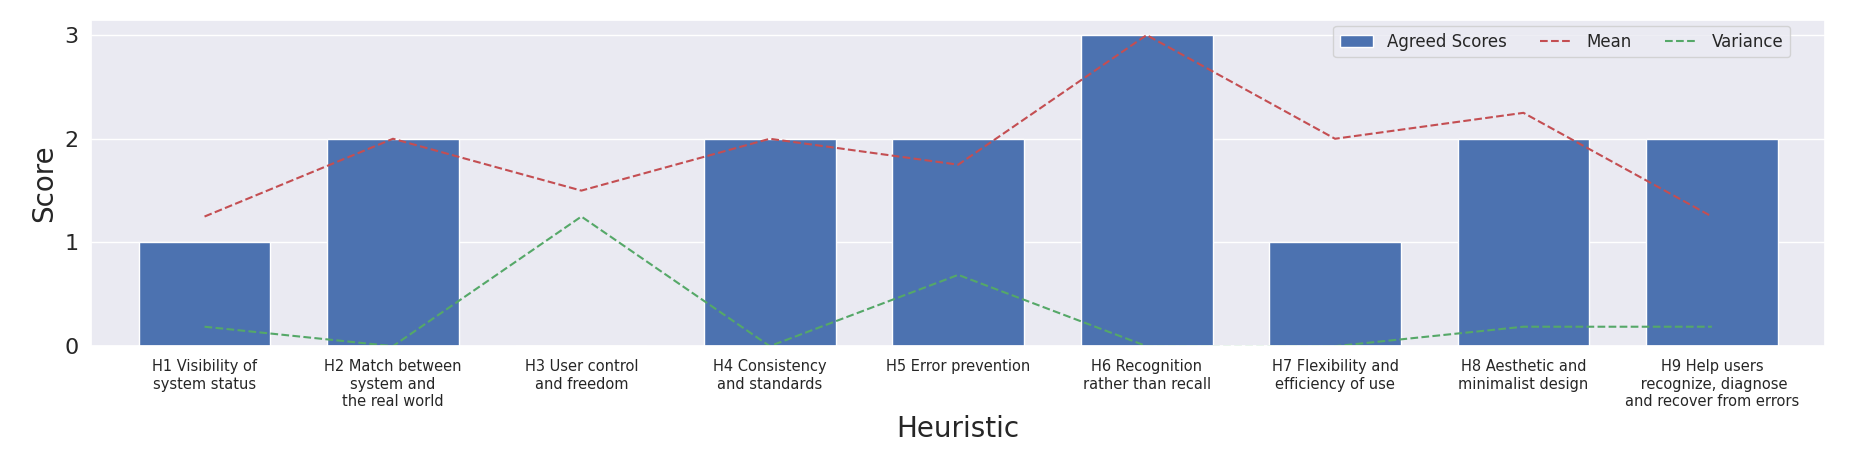
\includegraphics[width=1.2\textwidth]{images/BarsNielsenCrop.png}}%
        \captionsetup{justification=centering}
        \caption{Nielsen's heuristics evaluation summary}
        \label{BarsNielsenCrop}
    \end{minipage}
\end{figure}

\begin{figure}[!ht]
    \begin{minipage}{\linewidth}
        \centering
        \makebox[\textwidth][c]{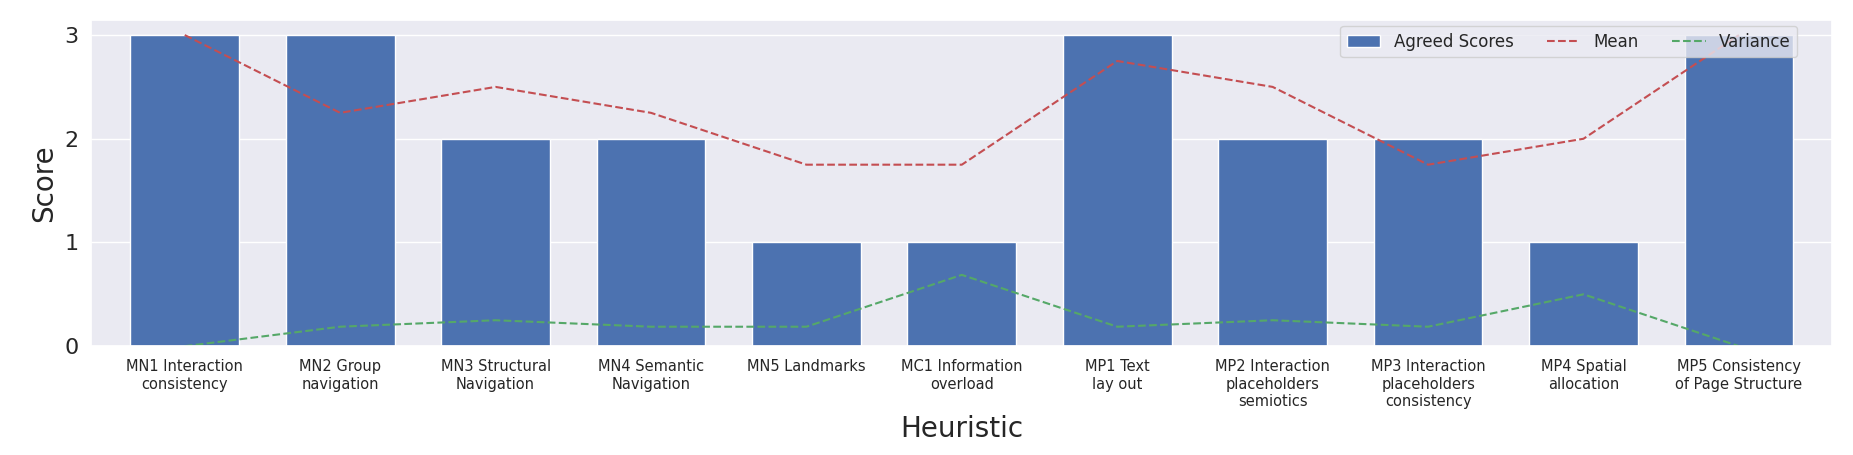
\includegraphics[width=1.2\textwidth]{images/BarsMileCrop.png}}%
        \captionsetup{justification=centering}
        \caption{MiLe's heuristics evaluation summary}
        \label{BarsMileCrop}
    \end{minipage}
\end{figure}

Mean values by content, navigation and presentation heuristics are provided in Fig \ref{BarsAggregated}.\\
There is an overall consensus that the website presents major problems on the content part. Explanations will be tackled in the next sections. 

\begin{figure}[!ht]
    \begin{minipage}{\linewidth}
        \centering
        \makebox[\textwidth][c]{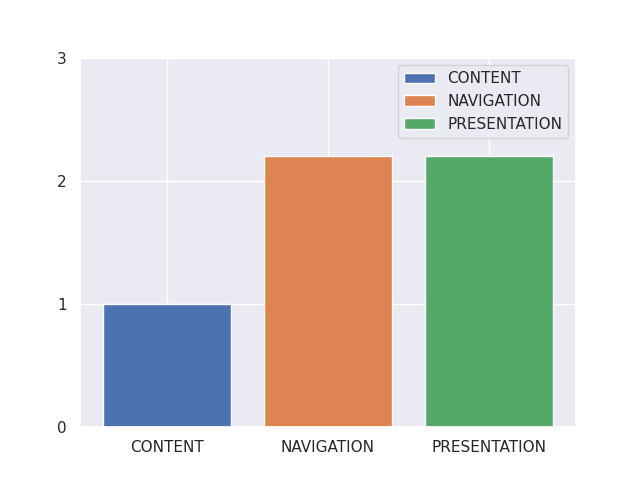
\includegraphics[width=0.6\textwidth]{images/BarsAggregated.png}}%
        \captionsetup{justification=centering}
        \caption{Aggregated heurstics data by dimensions}
        \label{BarsAggregated}
    \end{minipage}
\end{figure}

\pagebreak

\subsection{Discussion of results}
\subsubsection{Discussion within Nielsen's heuristics}
\begin{itemize}
    \item \textbf{H1 Visibility of system status}\\
    Commento su heuristic (Figura \ref{fig:1-image-ref})
    \begin{figure}[!ht]
        \begin{minipage}{\linewidth}
            \centering
            \captionsetup{justification=centering}
            \makebox[\textwidth][c]{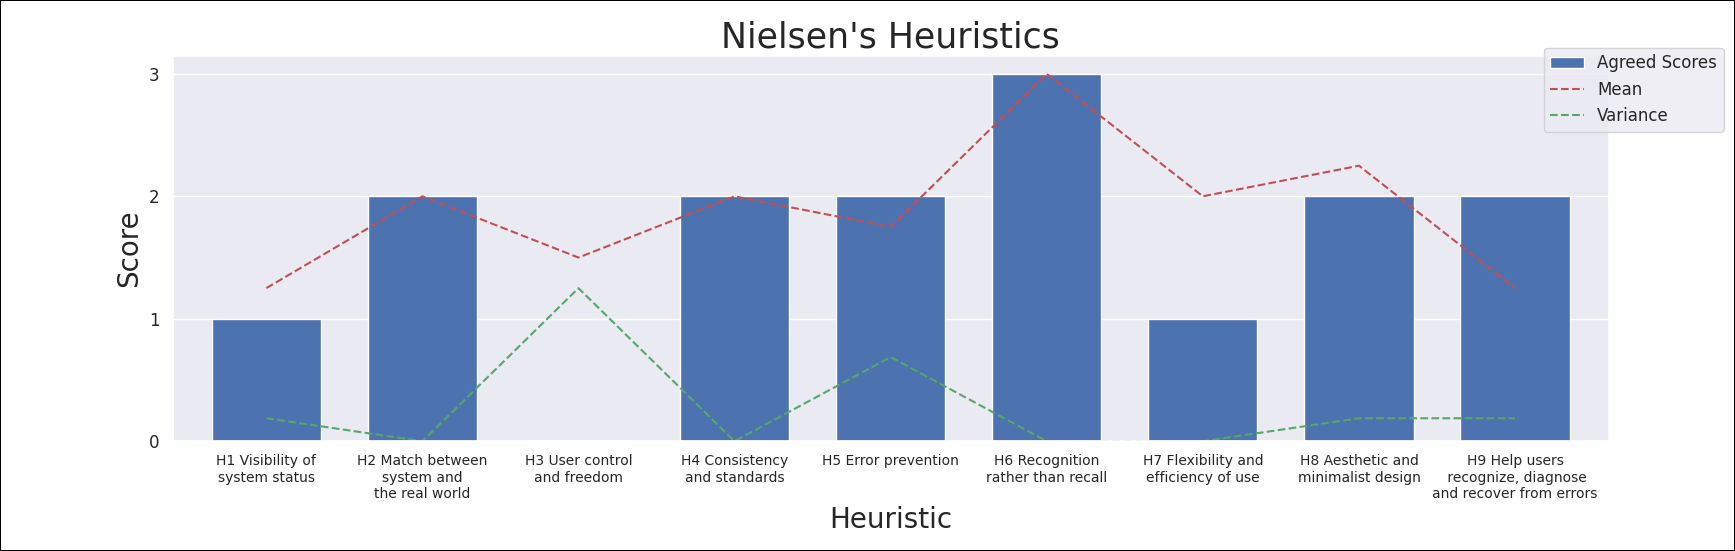
\includegraphics[width=0.7\textwidth]{images/test.png}}%
            \caption{Label dell'immagine}
            \label{fig:1-image-ref}
        \end{minipage}
    \end{figure}
    \item \textbf{H6 Recognition rather than recall}\\
    This heuristic is fully satisfied in fact all the search forms suggest options for recognition.
    \item \textbf{H7 Flexibility and efficiency of use}\\
    ???
    \item \textbf{H8 Aesthetic and minimalist design}\\
    Often, at the beginning of a page there's a big and useless image, thus requiring the user to scroll down in order to access some useful content. (See Fig. \ref{H8-1})\\
    In the page about the universities in Milan, there are very big images that could have been smaller. In fact it's difficult to have a good grasp of all the content, since lots of scrolling is needed. (See Fig. \ref{H8-2})
\begin{figure}[!ht]
            \begin{minipage}{\linewidth}
                \centering
                \makebox[\textwidth][c]{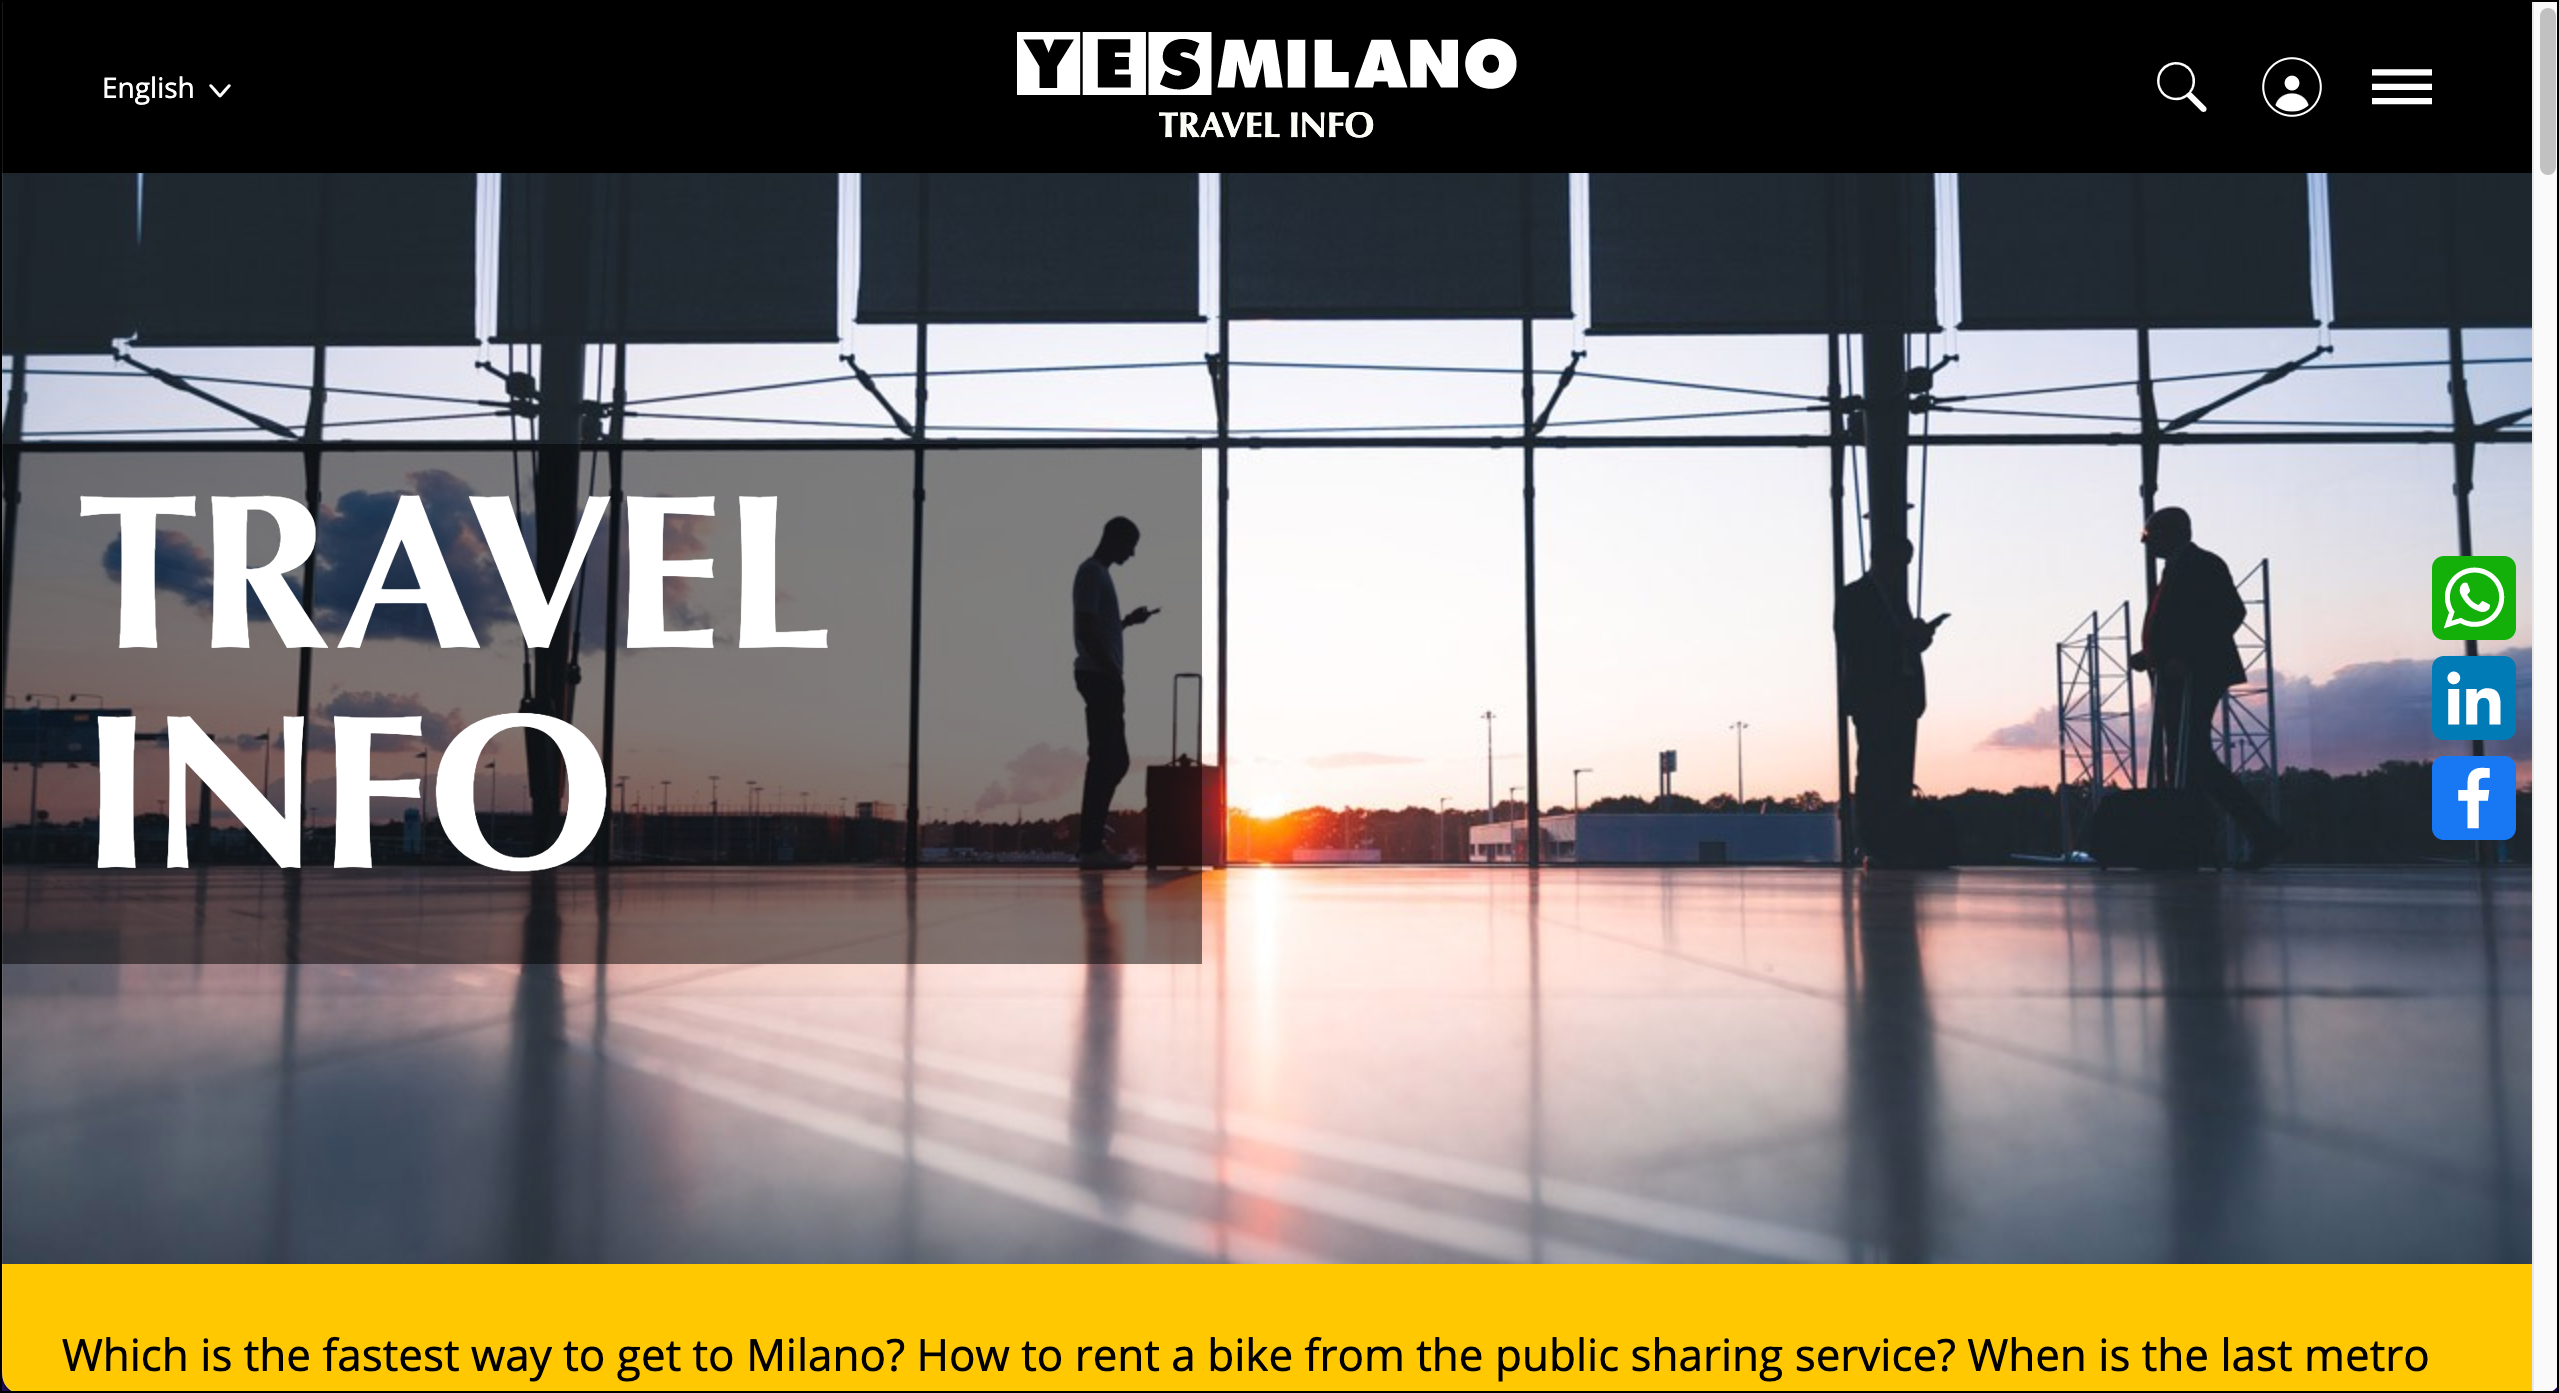
\includegraphics[width=0.5\textwidth]{images/H8-1.png}}%
                \captionsetup{justification=centering}
                \caption{}
                \label{H8-1}
            \end{minipage}
\end{figure}
\begin{figure}[!ht]
    \begin{minipage}{\linewidth}
        \centering
        \makebox[\textwidth][c]{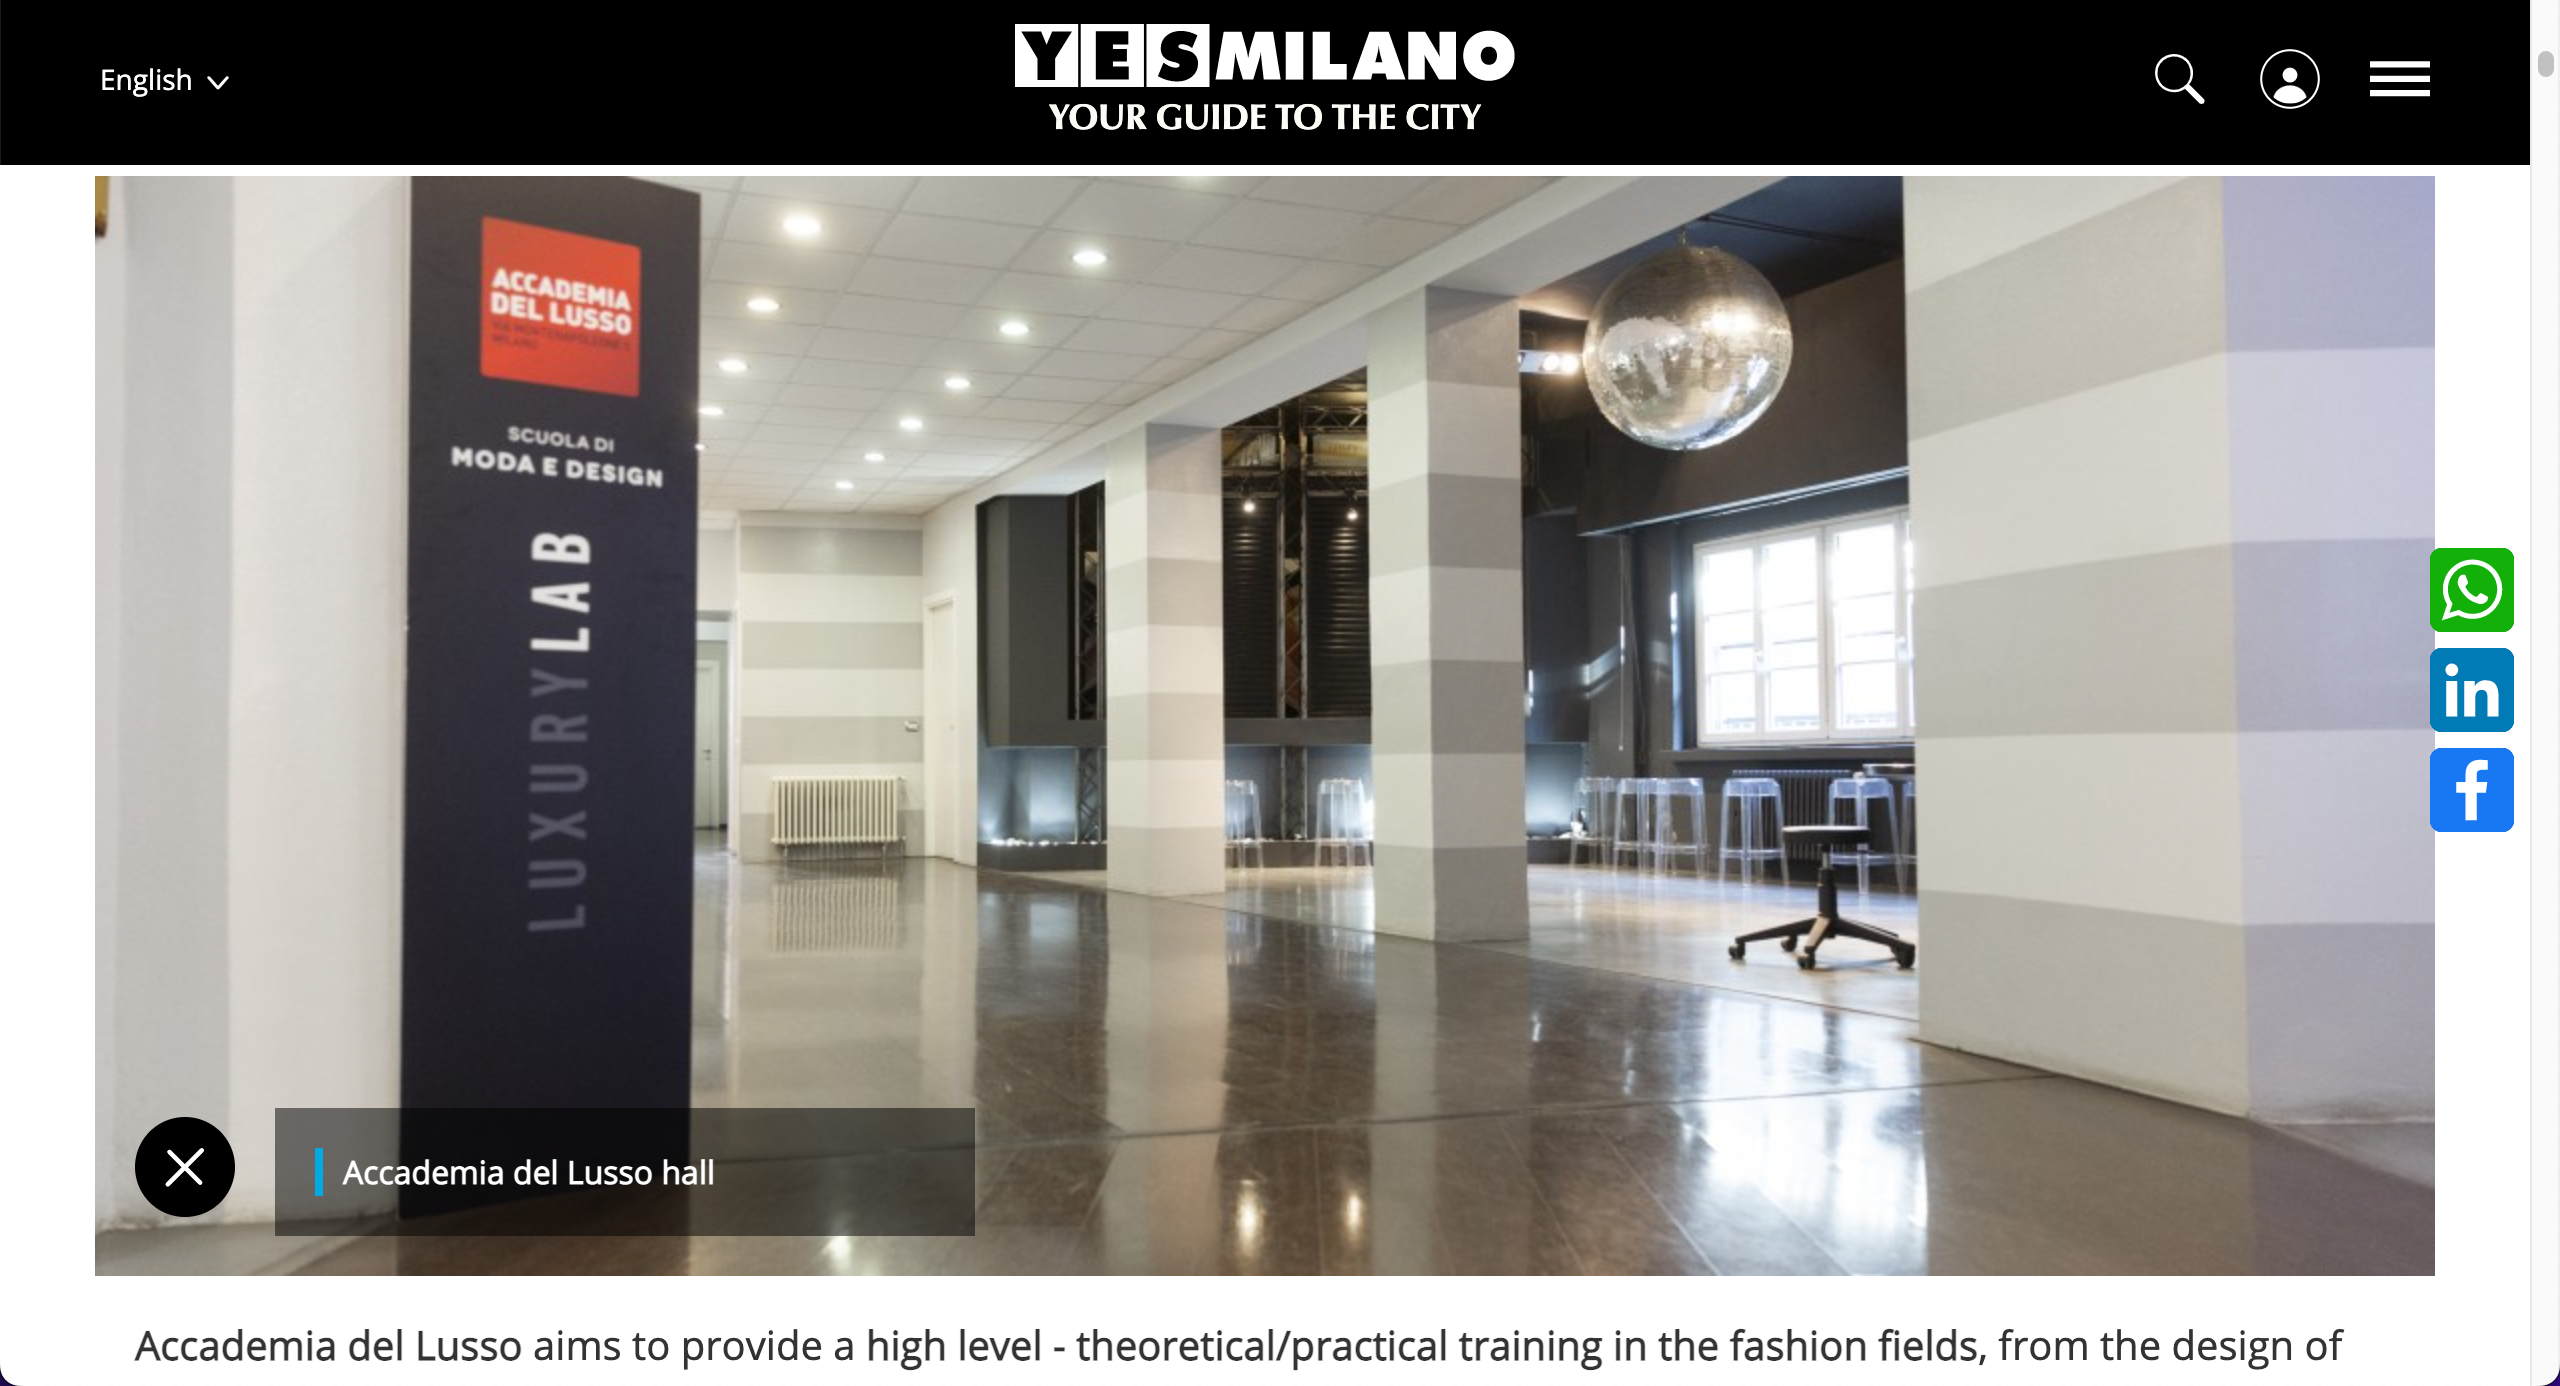
\includegraphics[width=0.5\textwidth]{images/H8-2.png}}%
        \captionsetup{justification=centering}
        \caption{}
        \label{H8-2}
    \end{minipage}
\end{figure}
    \item \textbf{H9 Help users recognize, diagnose and recover from errors}\\
    In the hotels page, if the geolocalization service fails, the website gives a not helpful error message (See Fig. \ref{H9-1}). Instead in the restaurants page, the same error gives to the user instructions about what to do. (See Fig. \ref{H9-2})\\
    When signing up for the newsletter, if the user first checks the checkbox then no error is shown for leaving the email field blank.\\
    The 404 error message is nicely designed. (See Fig. \ref{H9-3})\\
    The user form registration gives good error feedback. (See Fig. \ref{H9-4})
\begin{figure}[!ht]
        \begin{minipage}{\linewidth}
            \centering
            \makebox[\textwidth][c]{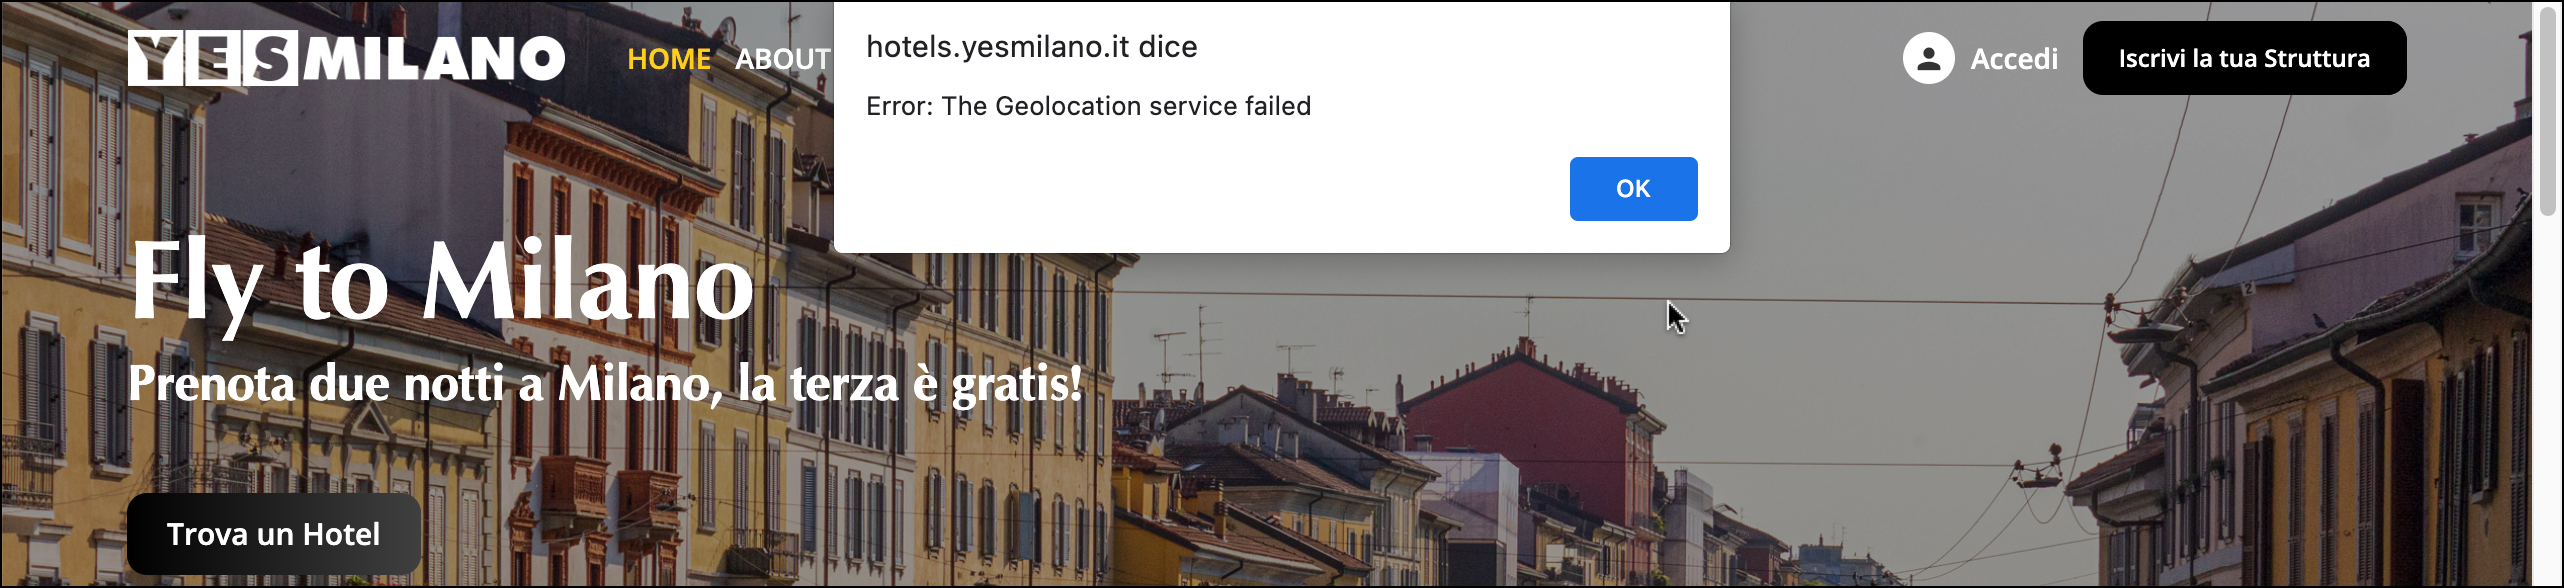
\includegraphics[width=0.5\textwidth]{images/H9-1.png}}%
            \captionsetup{justification=centering}
            \caption{}
            \label{H9-1}
        \end{minipage}
\end{figure}
\begin{figure}[!ht]
\begin{minipage}{\linewidth}
    \centering
    \makebox[\textwidth][c]{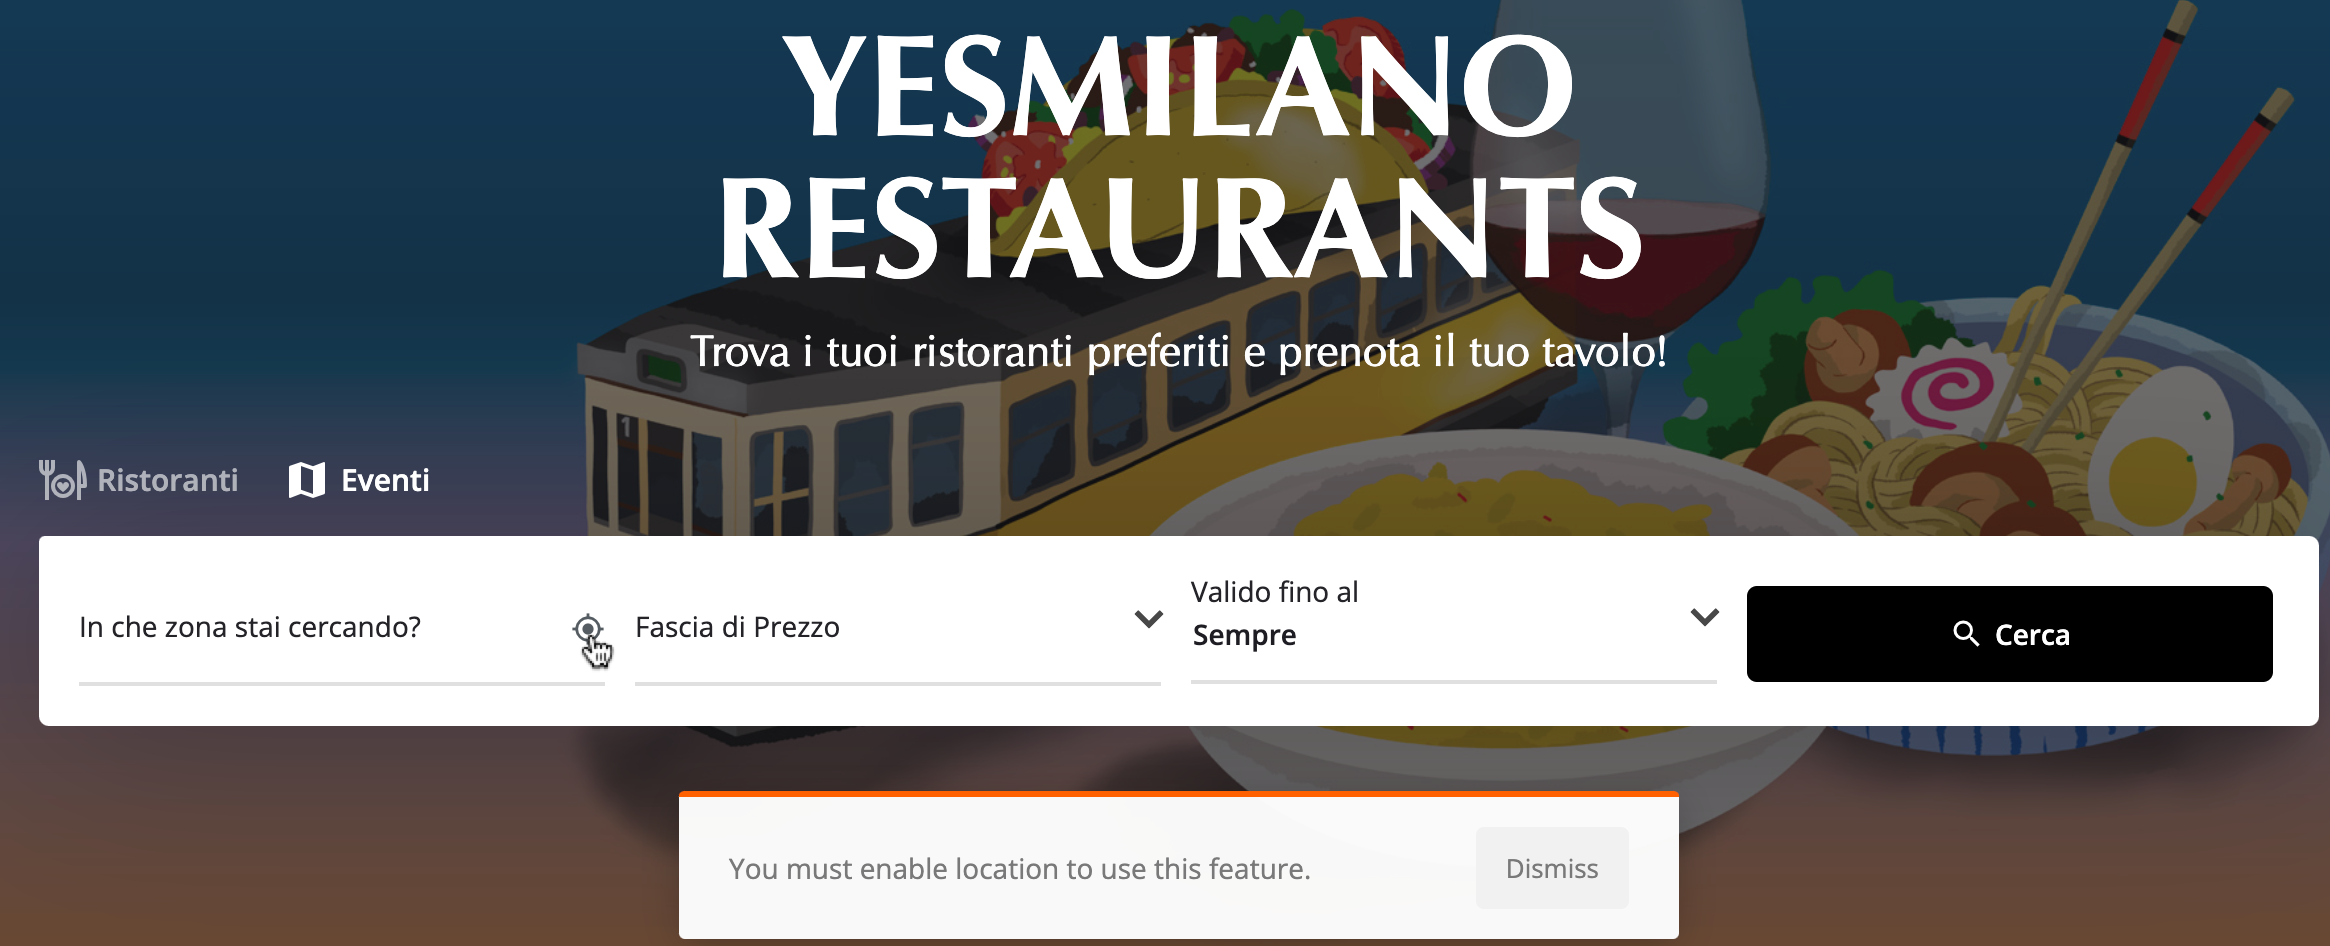
\includegraphics[width=0.5\textwidth]{images/H9-2.png}}%
    \captionsetup{justification=centering}
    \caption{}
    \label{H9-2}
\end{minipage}
\end{figure}\begin{figure}[!ht]
    \begin{minipage}{\linewidth}
        \centering
        \makebox[\textwidth][c]{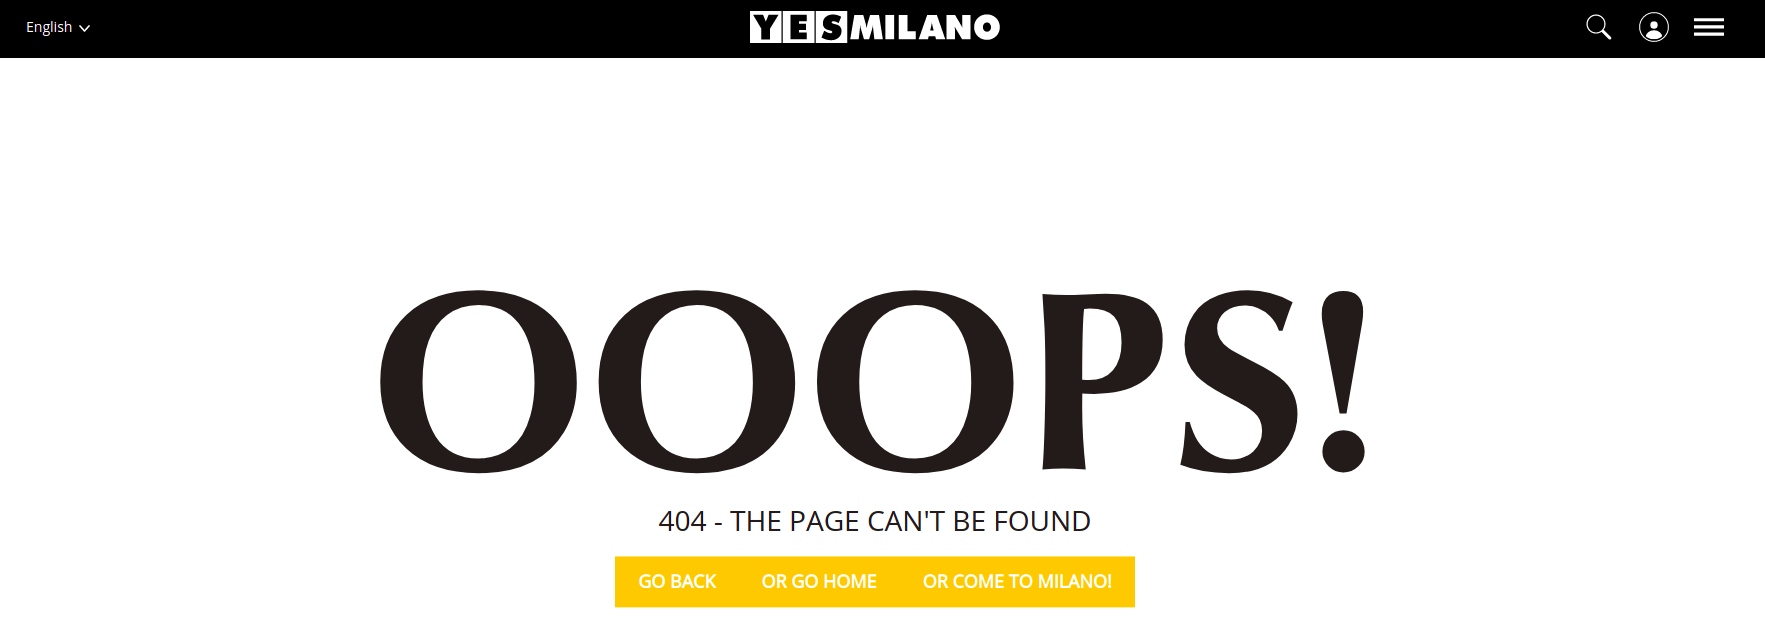
\includegraphics[width=0.5\textwidth]{images/H9-3.png}}%
        \captionsetup{justification=centering}
        \caption{}
        \label{H9-3}
    \end{minipage}
\end{figure}
\begin{figure}[!ht]
\begin{minipage}{\linewidth}
\centering
\makebox[\textwidth][c]{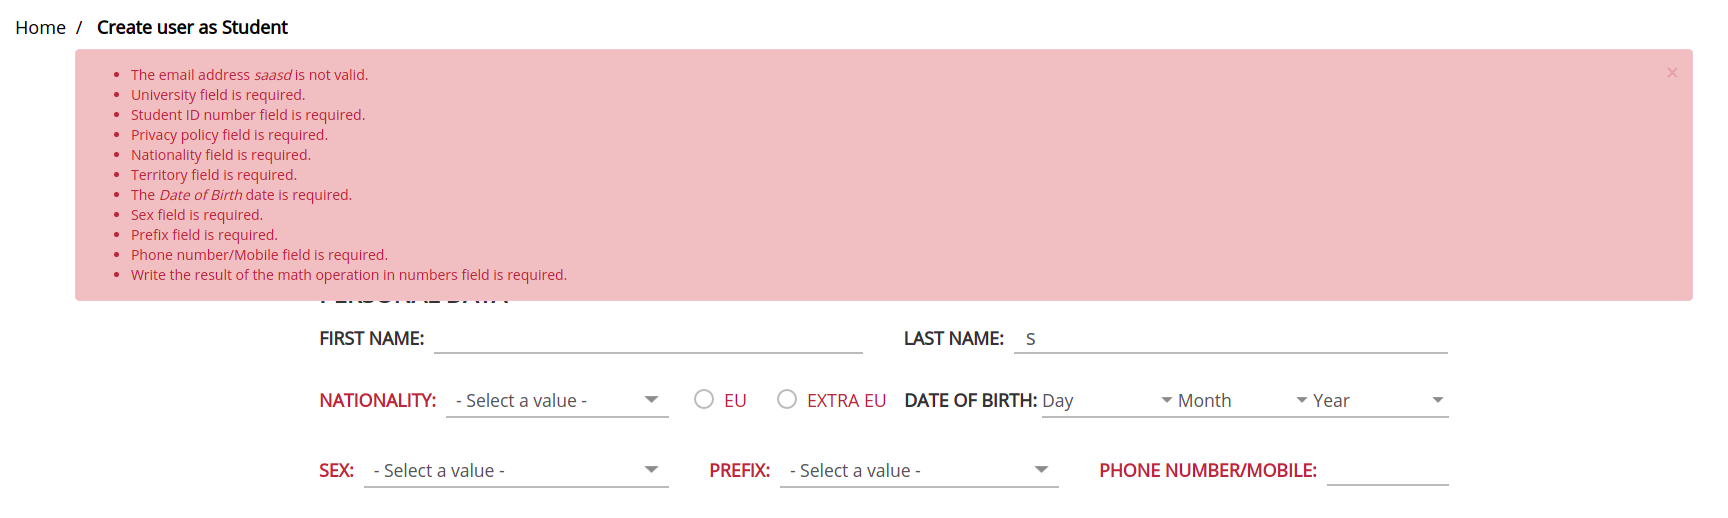
\includegraphics[width=0.5\textwidth]{images/H9-4.png}}%
\captionsetup{justification=centering}
\caption{}
\label{H9-4}
\end{minipage}
\end{figure}
    \item \textbf{H10 Help and documentation}\\
    N/A
\end{itemize}
\pagebreak
\subsubsection{Discussion within MiLe's heuristics}
\begin{itemize}
    \item \textbf{MN1 Interaction consistency}\\
    Similar pages have the same type of layout, links and interaction capabilities. Minor differences might be present, however they are not relevant.
    \item \textbf{MP1 Text lay out}\\
        No critical aspects found, the text is always readable and of the appropriate size.\\
    \item \textbf{MP2 Interaction placeholders-semiotics}\\
        Some minor problems were found in this heuristic: some icons are mismatched with regards to their meaning, and there are labels that are unclear in their functionalities (Fig. \ref{MP2-1} and \ref{MP2-2})
        \begin{figure}[!ht]
            \begin{minipage}{\linewidth}
                \centering
                \makebox[\textwidth][c]{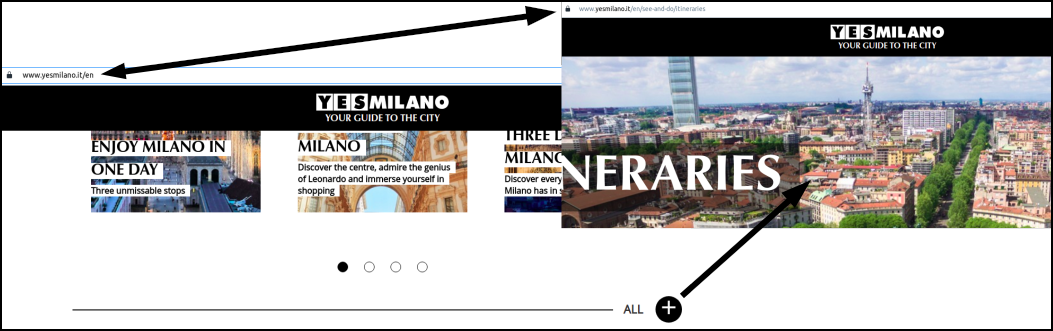
\includegraphics[width=1.2\textwidth]{images/MP2-1.png}}%
                \captionsetup{justification=centering}
                \caption{Conventionally, the "+" should expand the page,\\
                but in the home page it leads to a new page}
                \label{MP2-1}
            \end{minipage}
        \end{figure}
        \begin{figure}[!ht]
            \begin{minipage}{\linewidth}
                \centering
                \makebox[\textwidth][c]{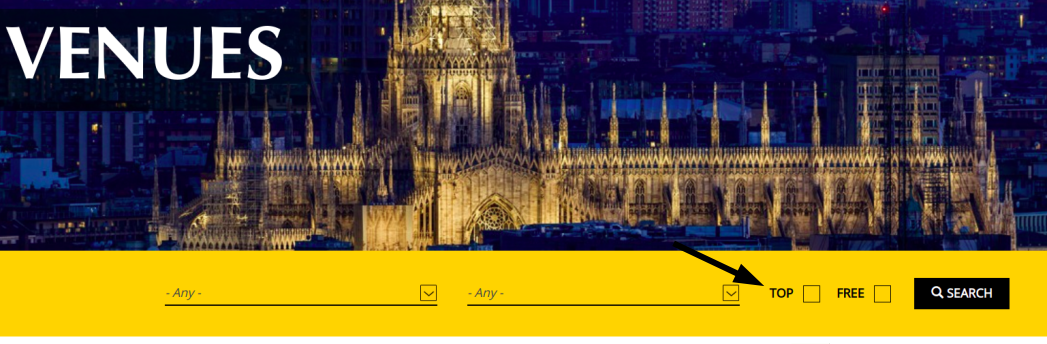
\includegraphics[width=1\textwidth]{images/MP2-2.png}}%
                \captionsetup{justification=centering}
                \caption{In the venues form page, it's unclear what does "TOP" mean in this context.\\If it's based on users reviews, there is no rating system explained}
                \label{MP2-2}
            \end{minipage}
        \end{figure}
    \item \textbf{MP3 Interaction placeholders-consistency}\\
        Some minor problems were found in this heuristic:
        a number of icons are used with multiple meanings (for example the "+" sometimes expands a paragraph section, other times it leads to a new page like in Fig \ref{MP2-1}), and many interactive labels providing the same functionalities are named differently across the same page (Fig \ref{MP3-1} and Fig \ref{MP3-2}).
        \begin{figure}[!ht]
            \begin{minipage}{\linewidth}
                \centering
                \makebox[\textwidth][c]{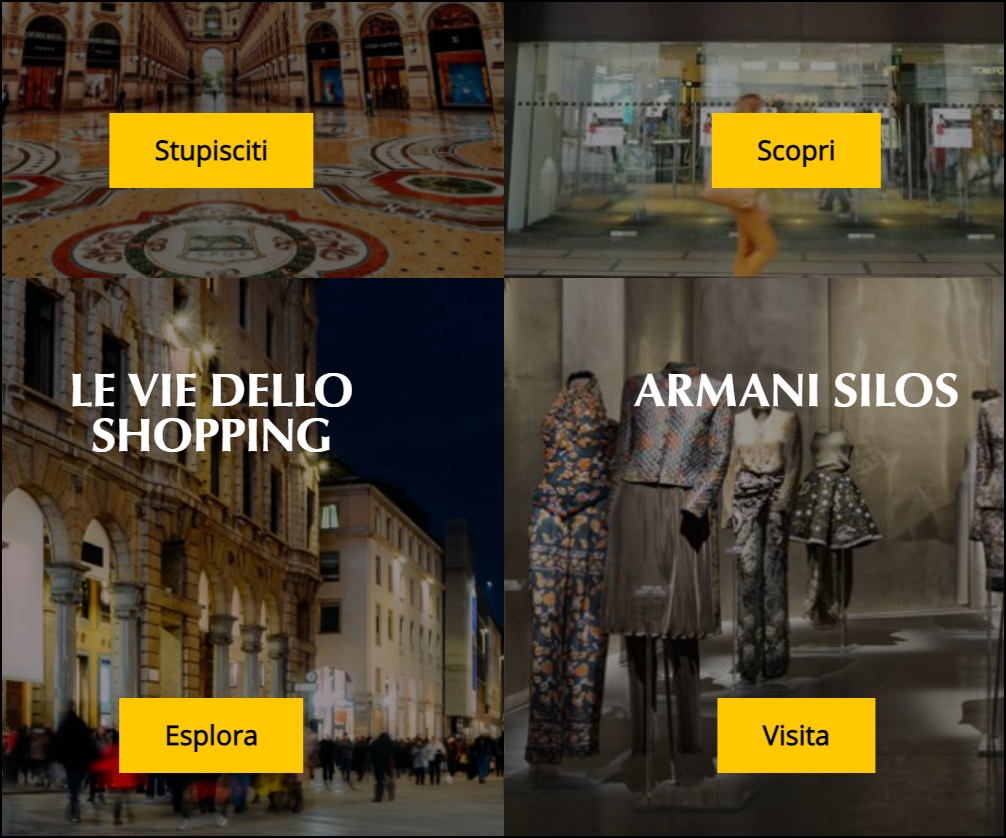
\includegraphics[width=0.5\textwidth]{images/MP3-1.png}}%
                \captionsetup{justification=centering}
                \caption{In the Fashion \& Shopping page, interactive labels are equivalent in terms of functionalities are named differently, sometimes even in confusing ways ("Stupisciti" which translates to "Amaze yourself" it's not really suggestive of its functionality)}
                \label{MP3-1}
            \end{minipage}
        \end{figure}
        \begin{figure}[!ht]
            \begin{minipage}{\linewidth}
                \centering
                \makebox[\textwidth][c]{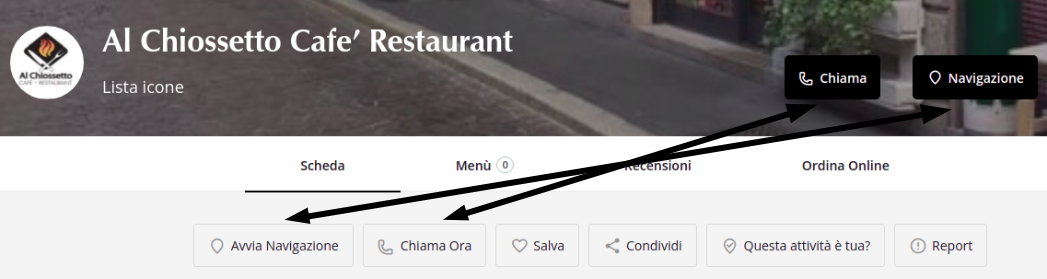
\includegraphics[width=1\textwidth]{images/MP3-2.png}}%
                \captionsetup{justification=centering}
                \caption{In any dedicated restaurant page, interactive elements\\for contacting and locating the place are labeled differently}
                \label{MP3-2}
            \end{minipage}
        \end{figure}
\end{itemize}

\pagebreak
Commento